\documentclass[11pt,a4paper]{article}

\usepackage[margin=1in]{geometry}
\usepackage{amsmath,amssymb}
\usepackage{booktabs}
\usepackage{array}
\usepackage{xcolor}
\usepackage{circuitikz}

\ctikzset{logic ports=american}

\title{COMP1003 Computer Organization\\Assignment 1}
\author{}
\date{}

\newcommand{\bin}[1]{\texttt{#1}}

\begin{document}
\maketitle
\thispagestyle{empty}

\section*{Q1}

\[
f(x,y,z)=x\cdot\bigl(y+\overline{z+x}\bigr)+\overline{z\cdot y}\cdot(x+z)
\]

\subsection*{(a) Truth table}

Each row is obtained by evaluating the two products and then OR-ing them.
Term~1 is \(x\cdot(y+\overline{z+x})\) and term~2 is \(\overline{z\cdot y}\cdot(x+z)\).

\begin{center}
\small
\setlength{\tabcolsep}{5pt}
\begin{tabular}{ccc ccc ccc c}
\toprule
\(x\) & \(y\) & \(z\)
  & \(\overline{z+x}\) & \(y+\overline{z+x}\) & term 1
  & \(\overline{zy}\) & \(x+z\) & term 2
  & \(f\) \\
\midrule
0 & 0 & 0 & 1 & 1 & 0 & 1 & 0 & 0 & 0 \\
0 & 0 & 1 & 0 & 0 & 0 & 1 & 1 & 1 & 1 \\
0 & 1 & 0 & 1 & 1 & 0 & 1 & 0 & 0 & 0 \\
0 & 1 & 1 & 0 & 1 & 0 & 0 & 1 & 0 & 0 \\
1 & 0 & 0 & 0 & 0 & 0 & 1 & 1 & 1 & 1 \\
1 & 0 & 1 & 0 & 0 & 0 & 1 & 1 & 1 & 1 \\
1 & 1 & 0 & 0 & 1 & 1 & 1 & 1 & 1 & 1 \\
1 & 1 & 1 & 0 & 1 & 1 & 0 & 1 & 0 & 1 \\
\bottomrule
\end{tabular}
\end{center}

\(f=1\) on minterms \(m_1,m_4,m_5,m_6,m_7\).

\subsection*{(b) Disjunctive normal form}

Reading the rows where \(f=1\):

\begin{align*}
f(x,y,z)
&= m_1+m_4+m_5+m_6+m_7 \\
&= \bar{x}\bar{y}z + x\bar{y}\bar{z} + x\bar{y}z + xy\bar{z} + xyz.
\end{align*}

\subsection*{(c) Karnaugh map}

Columns are in Gray-code order, so cells that share an edge differ in exactly one variable.

\begin{center}
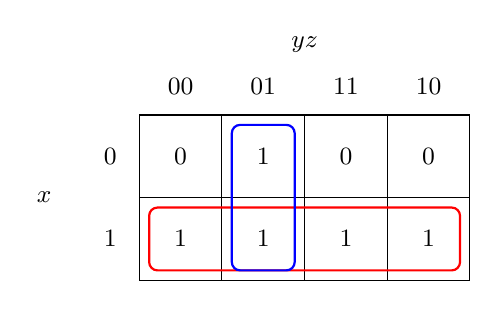
\begin{tikzpicture}[scale=1.05, every node/.style={font=\small}]
  \draw (0,0) grid (4,2);
  \node at (2,2.85) {\(yz\)};
  \node at (0.5,2.35) {00};
  \node at (1.5,2.35) {01};
  \node at (2.5,2.35) {11};
  \node at (3.5,2.35) {10};
  \node at (-1.15,1) {\(x\)};
  \node at (-0.35,1.5) {0};
  \node at (-0.35,0.5) {1};
  \node at (0.5,1.5) {0};
  \node at (1.5,1.5) {1};
  \node at (2.5,1.5) {0};
  \node at (3.5,1.5) {0};
  \node at (0.5,0.5) {1};
  \node at (1.5,0.5) {1};
  \node at (2.5,0.5) {1};
  \node at (3.5,0.5) {1};
  % quad: the whole x=1 row
  \draw[red, thick, rounded corners=3pt] (0.12,0.12) rectangle (3.88,0.88);
  % pair: column yz=01
  \draw[blue, thick, rounded corners=3pt] (1.12,0.12) rectangle (1.88,1.88);
\end{tikzpicture}
\end{center}

\begin{itemize}
  \item Red quad, the row \(x=1\): every cell is \(1\), so this group is \(x\).
  \item Blue pair, the column \(yz=01\): these two cells are \(\bar{y}z\).
    The cell \(x\bar{y}z\) belongs to both groups, which is allowed.
\end{itemize}

No \(1\) is left outside these groups, so
\[
f(x,y,z)=x+\bar{y}z.
\]

The same expression follows from the original formula.
By De~Morgan, \(\overline{z+x}=\bar{z}\,\bar{x}\) and \(\overline{zy}=\bar{z}+\bar{y}\), hence
\begin{align*}
f
&= x\bigl(y+\bar{x}\bar{z}\bigr)+(\bar{y}+\bar{z})(x+z) \\
&= xy + (\bar{y}x+\bar{y}z+x\bar{z}) \\
&= x(y+\bar{y})+\bar{y}z+x\bar{z} \\
&= x+\bar{y}z,
\end{align*}
where \(x+x\bar{z}=x\).

\subsection*{(d) Logic circuit of the minimized function}

\(f=x+\bar{y}z\) uses one NOT, one AND, and one OR.

\begin{center}
\begin{circuitikz}[scale=1.05]
  \draw (0,0) node[not port] (ny) {}
        (ny.out) -- ++(0.6,0)
        node[and port, anchor=in 1] (a) {}
        (ny.in) node[left] {\(y\)}
        (a.in 2) node[left] {\(z\)}
        (a.out) -- ++(0.7,0)
        node[or port, anchor=in 2] (o) {}
        (o.in 1) node[left] {\(x\)}
        (o.out) node[right] {\(f\)};
\end{circuitikz}
\end{center}

\section*{Q2}

\subsection*{(a) \(152_{\mathrm{dec}}\) to binary}

Divide by \(2\) and record the remainders. The binary digits are those remainders read from last to first.

\begin{center}
\begin{tabular}{r@{\;}c@{\;}l@{\qquad}l}
\(152\) & \(=\) & \(2\cdot 76+0\) & remainder \(0\) \\
\(76\)  & \(=\) & \(2\cdot 38+0\) & remainder \(0\) \\
\(38\)  & \(=\) & \(2\cdot 19+0\) & remainder \(0\) \\
\(19\)  & \(=\) & \(2\cdot 9+1\)  & remainder \(1\) \\
\(9\)   & \(=\) & \(2\cdot 4+1\)  & remainder \(1\) \\
\(4\)   & \(=\) & \(2\cdot 2+0\)  & remainder \(0\) \\
\(2\)   & \(=\) & \(2\cdot 1+0\)  & remainder \(0\) \\
\(1\)   & \(=\) & \(2\cdot 0+1\)  & remainder \(1\) \\
\end{tabular}
\end{center}

\[
152_{\mathrm{dec}}=10011000_{2}.
\]
Check: \(2^{7}+2^{4}+2^{3}=128+16+8=152\).

\subsection*{(b) Unsigned \(11001010_{\mathrm{bin}}\) to decimal}

\[
\begin{aligned}
11001010_{2}
&= 2^{7}+2^{6}+2^{3}+2^{1} \\
&= 128+64+8+2 \\
&= 202_{\mathrm{dec}}.
\end{aligned}
\]

\subsection*{(c) Signed \(11001010_{\mathrm{sig}}\) to decimal}

The subscript \(\mathrm{sig}\) is read as sign-magnitude.
Part~(d) asks for two's complement separately, so the sign bit here is not a two's-complement sign.

The leading bit is \(1\), so the number is negative.
The magnitude is the remaining seven bits:
\[
1001010_{2}=2^{6}+2^{3}+2^{1}=64+8+2=74.
\]
Therefore
\[
11001010_{\mathrm{sig}}=-74_{\mathrm{dec}}.
\]

(The same eight bits, if they were instead an 8-bit two's-complement integer, would equal \(-54\). That reading is not used here.)

\subsection*{(d) \(-152_{\mathrm{dec}}\) as 8-bit two's complement}

An \(n\)-bit two's-complement integer lies in \([-2^{n-1},\,2^{n-1}-1]\).
For \(n=8\) the interval is \([-128,127]\).
Since \(-152<-128\), \(-152\) has no 8-bit two's-complement representation.

The shortest width that contains it is \(9\) bits, whose range is \([-256,255]\).
Start from the positive value and apply invert-and-add-one:
\[
\begin{aligned}
+152 &= 0\,1001\,1000_{2}, \\
\text{invert} &= 1\,0110\,0111_{2}, \\
+1 &= 1\,0110\,1000_{2}.
\end{aligned}
\]
So the 9-bit two's-complement form is \(101101000_{2}\).
Inverting that pattern and adding one recovers \(010011000_{2}=152\), which confirms the sign.

\subsection*{(e) \(FACE_{\mathrm{hex}}\) to octal}

Replace each hex digit by four bits, then regroup by three bits from the right.

\[
\begin{aligned}
F&=1111, & A&=1010, & C&=1100, & E&=1110, \\
FACE_{16}&=1111\,1010\,1100\,1110_{2}.
\end{aligned}
\]
\[
1\,111\,101\,011\,001\,110_{2}=175316_{8}.
\]
Decimal check: \(15\cdot16^{3}+10\cdot16^{2}+12\cdot16+14=64206\), and \(64206_{10}=175316_{8}\).

\subsection*{(f) Half-precision \(1011001110001100\) to decimal}

IEEE~754 binary16 has \(1\) sign bit, \(5\) exponent bits (bias \(15\)), and \(10\) fraction bits:
\[
1\;\;01100\;\;1110001100.
\]

\begin{itemize}
  \item Sign bit \(1\): the value is negative.
  \item Stored exponent \(01100_{2}=12\). It is neither \(00000\) nor \(11111\), so the number is normal.
        The true exponent is \(12-15=-3\), and the leading significand bit is \(1\).
  \item Fraction \(1110001100_{2}=908\), so
        \[
        1+\frac{908}{1024}
        =1+\frac{227}{256}
        =\frac{483}{256}.
        \]
\end{itemize}

\[
\begin{aligned}
1011001110001100
&= -\frac{483}{256}\cdot 2^{-3} \\
&= -\frac{483}{2048} \\
&= -0.23583984375_{\mathrm{dec}}.
\end{aligned}
\]

\section*{Q3}

Unsigned integers, with no fixed word size:
\[
1111001_{2}\times 10011_{2}-1010110_{2}.
\]

\subsection*{(a) Binary value}

The multiplier bits, from the right, are \(1,1,0,0,1\).
The two zero partial products are omitted; the three nonzero ones are shifted by \(0\), \(1\), and \(4\) places.

\[
\begin{array}{r@{\;}r}
 & 1111001 \\
\times & 10011 \\
\hline
 & 1111001 \\
 & 1111001\phantom{0} \\
 & 1111001\phantom{0000} \\
\hline
 & 100011111011
\end{array}
\]

The first two partial products add as
\[
1111001_{2}+11110010_{2}=101101011_{2},
\]
and
\[
101101011_{2}+11110010000_{2}=100011111011_{2}.
\]

Subtract the third operand. Align \(1010110_{2}\) on the right:
\[
\begin{array}{r}
  100011111011 \\
-\phantom{1}00001010110 \\
\hline
  100010100101
\end{array}
\]
The only borrow starts at bit~2 (value bits numbered from \(0\) on the right): that bit is \(0-1\), so it borrows from bit~3 and the result bit is \(1\). No further borrow is generated. The remaining bits subtract directly and give \(100010100101_{2}\).

\[
1111001_{2}\times 10011_{2}-1010110_{2}=100010100101_{2}.
\]

\subsection*{(b) Decimal check}

\[
\begin{aligned}
1111001_{2}&=64+32+16+8+1=121, \\
10011_{2}&=16+2+1=19, \\
1010110_{2}&=64+16+4+2=86.
\end{aligned}
\]
\[
121\times 19-86=2299-86=2213.
\]
\[
2213=2^{11}+2^{7}+2^{5}+2^{2}+2^{0}=100010100101_{2},
\]
which matches part~(a).

\end{document}
